
\begin{appendix}

  \section{Extra Pictures}

  \begin{figure}[!htbp]
    \centering
    \begin{subfigure}[b]{1\textwidth}
      \includegraphics[width=\textwidth]{img/part1/LSTM_train_t5_lr_1e-2.png}
      \caption{Learning Rate $1\mathrm{e}^{-2}$}
    \end{subfigure}
    \begin{subfigure}[b]{1\textwidth}
      \includegraphics[width=\textwidth]{img/part1/LSTM_train_t5_lr_1e-4.png}
      \caption{Learning Rate $1\mathrm{e}^{-4}$}
    \end{subfigure}
    \caption{$T = 5$ Change Learning Rate Curve}
    \label{fig:p1_t5_lr_change}
  \end{figure}

  \begin{figure}[!htbp]
    \centering
    \begin{subfigure}[b]{1\textwidth}
      \includegraphics[width=\textwidth]{img/part1/LSTM_train_t20_lr_1e-2.png}
      \caption{Learning Rate $1\mathrm{e}^{-2}$}
    \end{subfigure}
    \begin{subfigure}[b]{1\textwidth}
      \includegraphics[width=\textwidth]{img/part1/LSTM_train_t20_lr_1e-4.png}
      \caption{Learning Rate $1\mathrm{e}^{-4}$}
    \end{subfigure}
    \caption{$T = 20$ Change Learning Rate Curve}
    \label{fig:p1_t20_lr_change}
  \end{figure}

  \begin{figure}[!htbp]
    \centering
    \includegraphics[width=1\textwidth]{img/part1/LSTM_train_t30_lr_1e-4.png}
    \caption{$T = 30$ Learning Rate $1\mathrm{e}^{-4}$ Curve}
    \label{fig:p1_t30}
  \end{figure}

  \begin{figure}[!htbp]
    \centering
    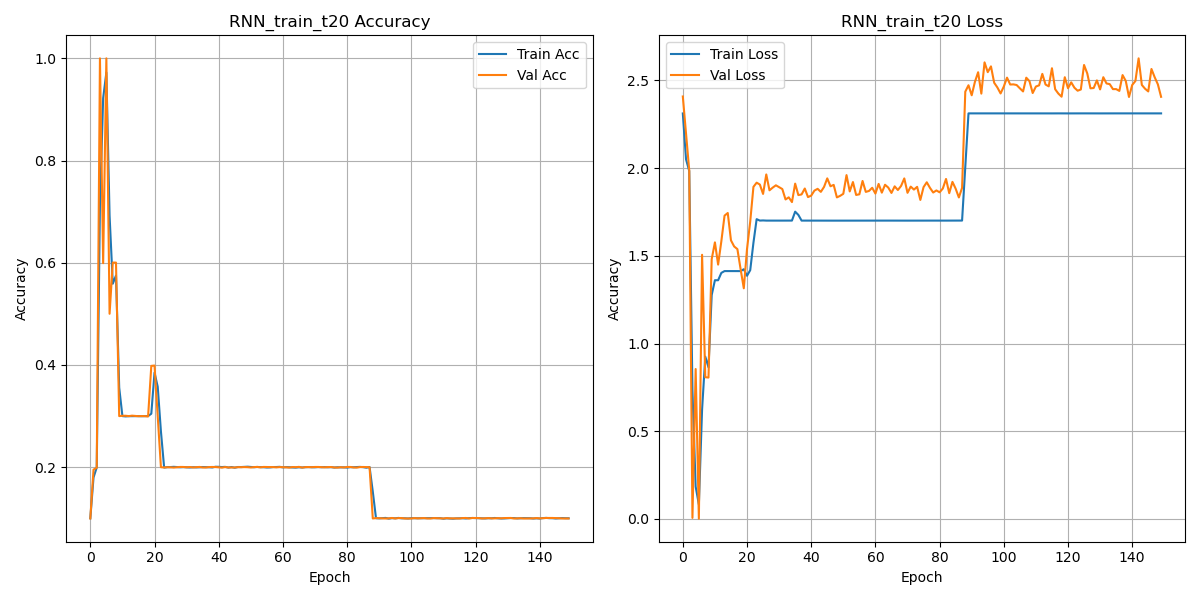
\includegraphics[width=1\textwidth]{img/part1/RNN_train_t20_default.png}
    \caption{$T = 20$ RNN Curve}
    \label{fig:p1_t20_rnn}
  \end{figure}

\end{appendix}
